\begin{par}
    \subsubsection{Classification Result Using Mel-Frequency Cepstral Coefficient}
    \par \hspace{15pt} In order to retain an acceptable time-efficiency for the singular value decomposition required in the team's Sub-space Learning (SL) module, the team needs to shrink down the size of the song tracks. One challenge for this task is that the compression must make sure the prominent features of the song data stay distinguishable so an effective classification is possible. With this in mind, the team decides to adopt a feature extraction/representation method called Mel-Frequency Cepstral Coefficient (MFCC) in order to take out the most prominent patterns of the songs.
    \par MFCC is originally used to represent the power-spectrum of an acoustic signal. Since the coefficients of MFC are able to represent the frequency features (after applying Fourier transform) of the signal, this quantity is widely used in audio compression. Although the MFCC is originally designed to transform a time-amplitude signal, and that our data set are binary values, with pitch instead of amplitude of the sound recorded at each time-step, the team can still take advantage of its ability to describe the noticeable shape and patterns of a signal-the song tracks can be seen as time-amplitude signal where the amplitude equals, in numeric value, to the pitch at each time-step.
    \par The team tries to use the sets of MFCC for each song track instead of Pianoroll binary data before Mel-Frequency Cepstral transformation. The parameters used for calculating MFCC are the following: Sample-rate = 8000 Hz, Window length = 0.025, Window step = 0.01, Number of Cepstral Coefficient = 16, Number of Filters = 26. The sample-rate needs to be the power of 2, and it should reflect the frequency at which the sound signal is collected; the calculation of MFCC segments the sound signal into multiple pieces called "window", so the window length determines the length of each piece, while the window step determines the distance between two windows; therefore, decreasing window step increases the total number of MFCC calculated. Using MFCC as inputs to the subspace learning method, the team obtains a classification accuracy of 45 percent; a sample singular value plot is shown in Figure \ref{mfcc_svd} transforming the original data into MFCC matrices elevate the classification accuracy from 10 to 45 percent.

\end{par}
\begin{par}
    \begin{figure}[H]
        \centering
        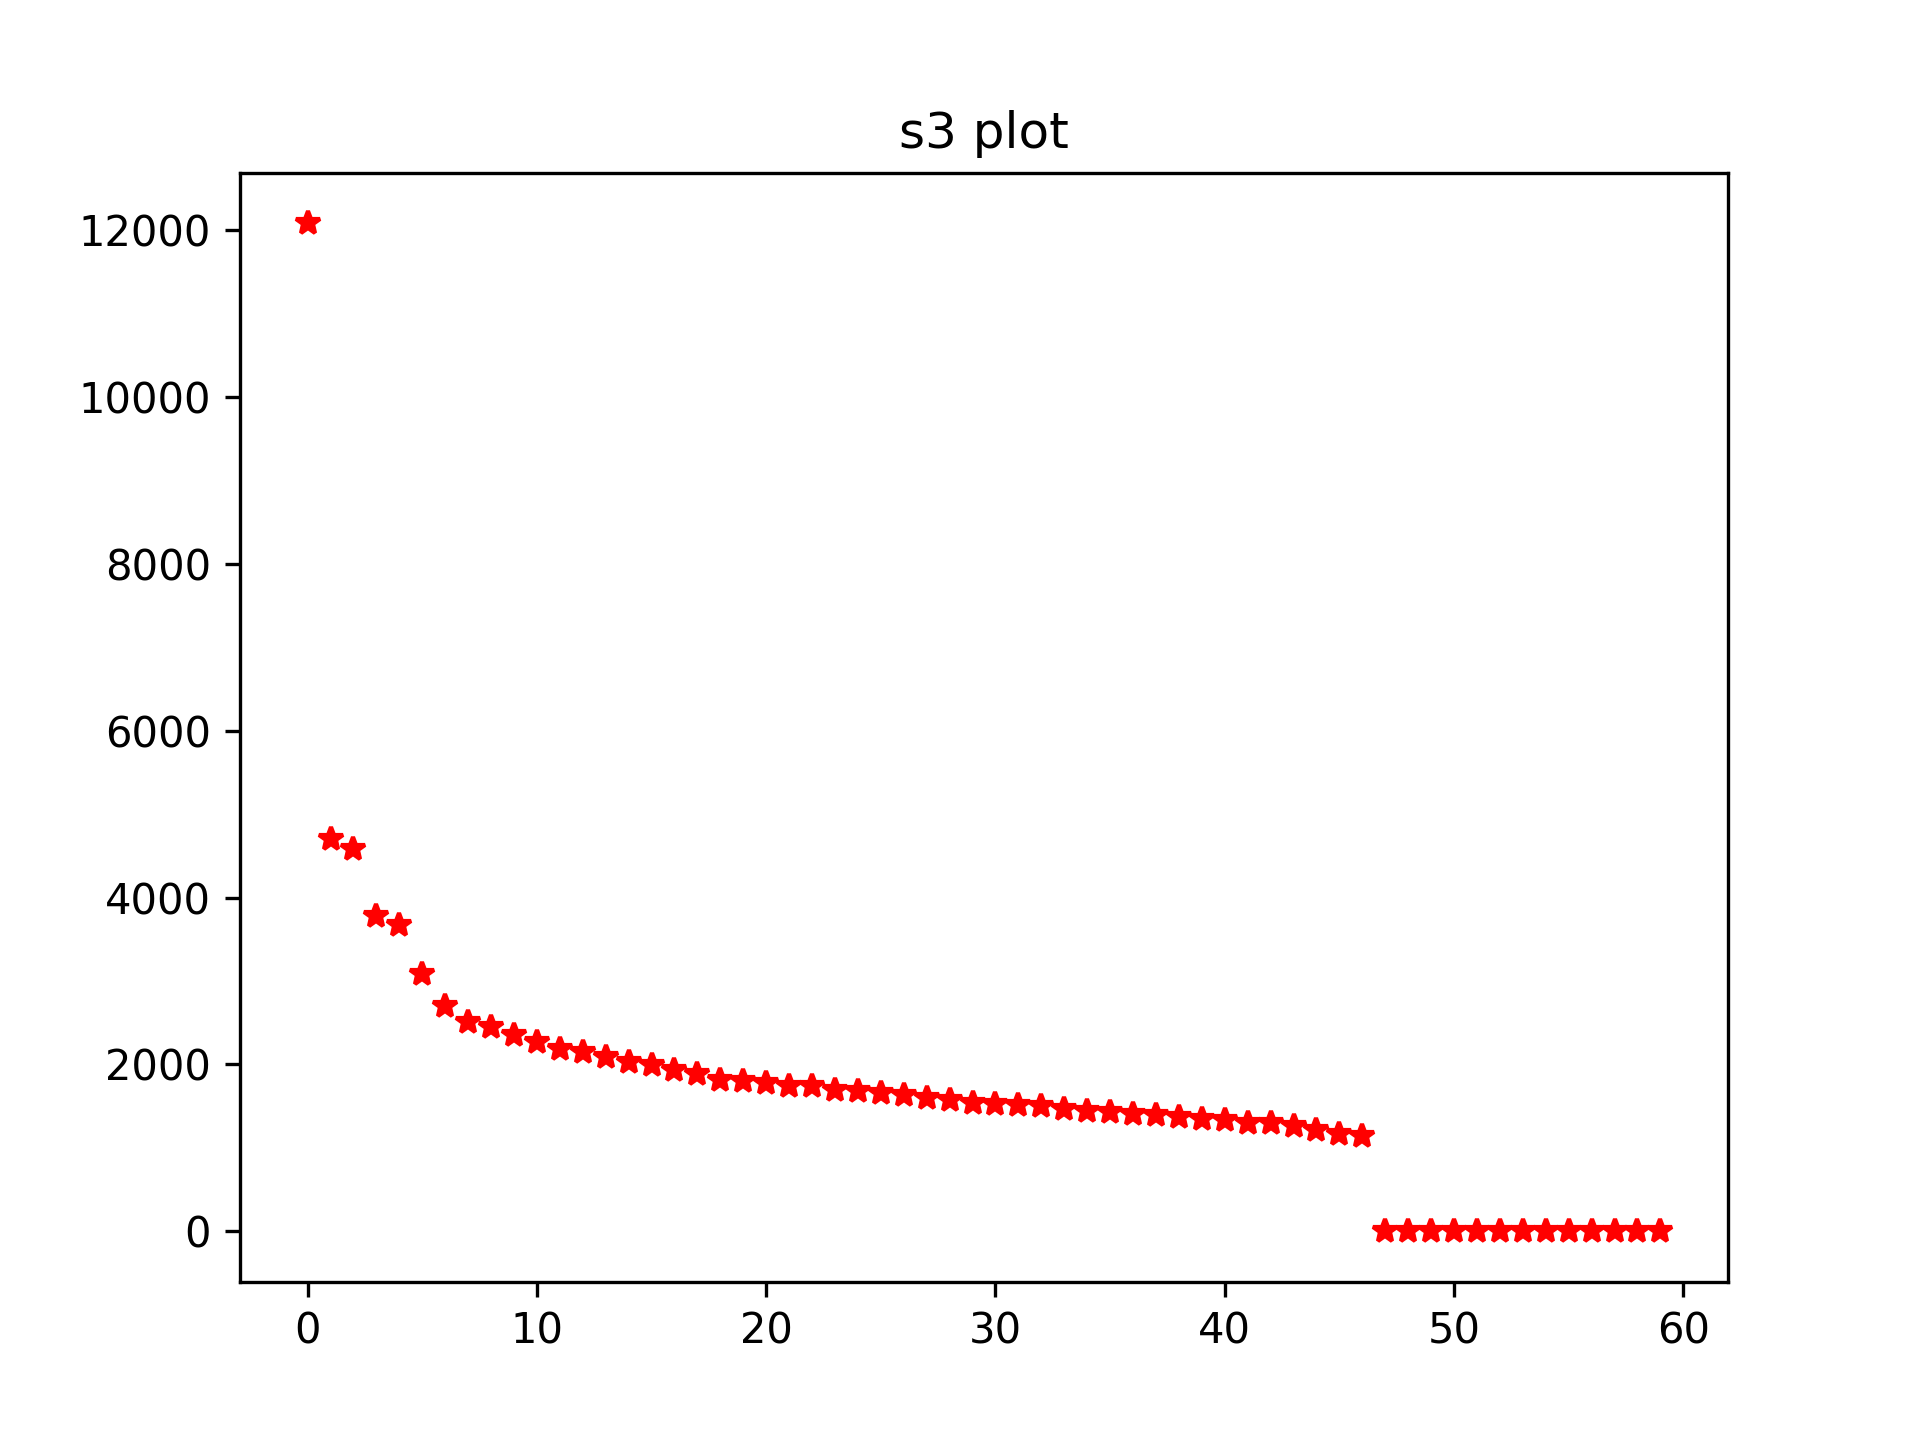
\includegraphics[width=4in]{image/s3_plot_mfcc.png}
        \caption{Singular Value Plot for Genre 3 (MFCC)}
        \label{fig:mfcc_svd}
    \end{figure}
    \end{par}